\section{Theoretical Analysis}
\label{sec:analysis}

In this section, the circuit depicted in Figure~\ref{circuit} is analysed with two different methods, so as to determine how it behaves, theoretically, both in terms of current in each branch and potential difference between nodes.

\subsection{Mesh analysis method}

The first method considered is the Mesh analysis method, considering the four meshes present in the circuit. Each mesh is given a label ($\alpha$, $\beta$, $\gamma$ and $\delta$) and an arbitrary direction for the current to flow in, as the below figure shows.

\begin{figure}[H]
  \centering
  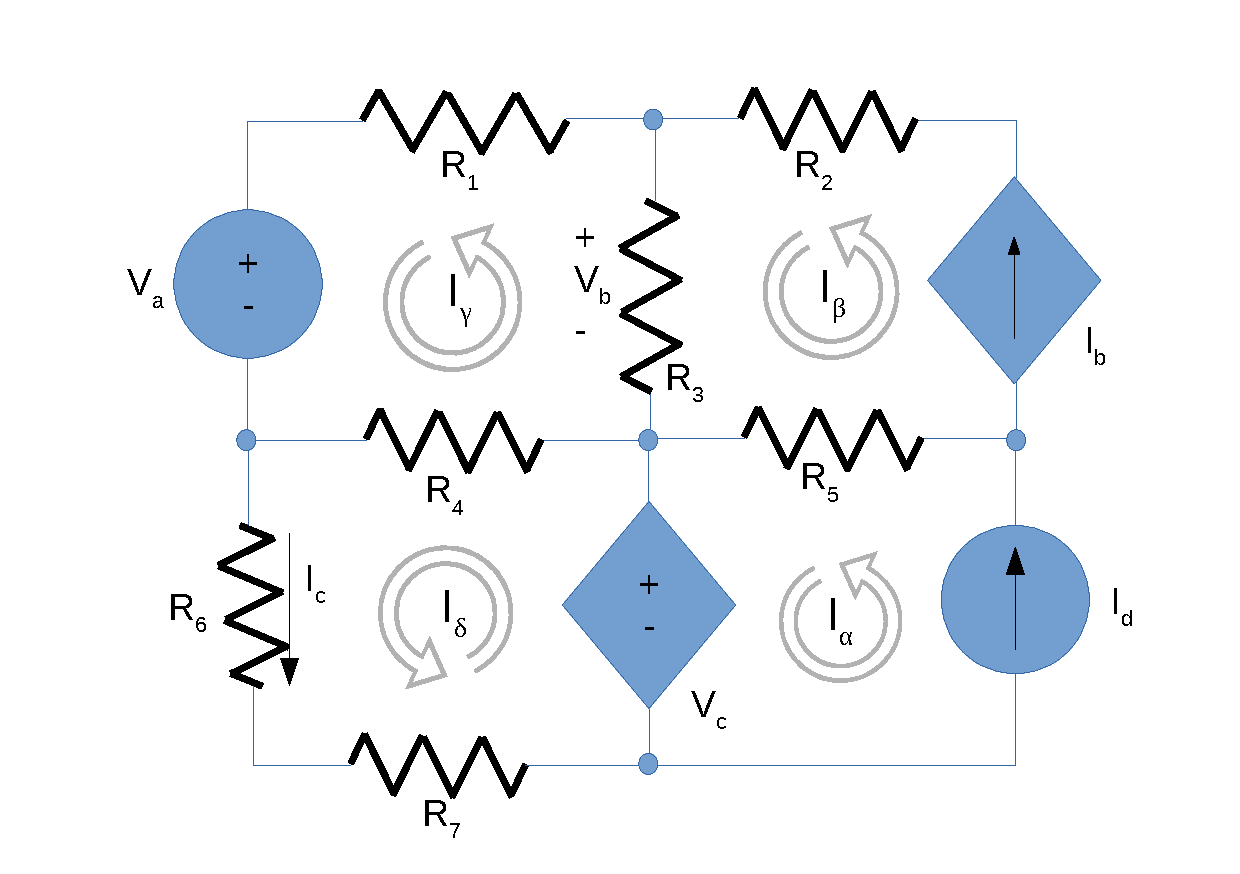
\includegraphics[width=0.8\linewidth]{mesh.pdf}
  \caption{Mesh analysis}
  \label{mesh_fig}
\end{figure}

By inspection:

\begin{equation}
  \begin{cases}
    I_{\alpha} = I_d \\
    I_{\beta} = I_b
  \end{cases}
\end{equation}

Applying KVL to the two remaining meshes:

\begin{equation}
  \begin{cases}
    V_a + R_4 (I_\gamma + I_\delta) + R_3 (I_\gamma - I_\beta) + R_1 I_\gamma = 0 \\
    V_c + R_7 I_\delta + R_6 I_\delta + R_4 (I_\delta + I_\gamma) = 0
  \end{cases}
\end{equation}

The conditional sources behave as:

\begin{equation}
  \begin{cases}
  I_b = k_b V_b \\
  V_c = k_c I_c = - k_c I_\delta
  \end{cases}
\end{equation}

Lastly, by Ohm's Law

\begin{equation}
  V_b = R_3 (I_\beta - I_\gamma)
\end{equation}

Manipulating these equations and solving them using Octave yields:

%\begin{equation}
%  \begin{bmatrix}
%  1 & 0 & 0 & 0 \\
%  0 & 1-k_b R_3 & k_b R_3 & 0 \\
%  0 & -R_3 & R_1+R_3+R_4 & R_4 \\
%  0 & 0 & R_4 & R_4+R_6+R_7-k_c
%  \end{bmatrix}
%  \begin{bmatrix}
%  I_\alpha \\
%  I_\beta \\
%  I_\gamma \\
%  I_\delta
%  \end{bmatrix}
%  =
%  \begin{bmatrix}
%  I_d \\
%  0 \\
%  -V_a \\
%  0
%  \end{bmatrix}
%\end{equation}

%Solving this system using Octave,

\begin{table}[H]
  \centering
  \begin{tabular}{|c|c|}
    \hline
        {\bf Name} & {\bf Value} \\
        \hline
        \hline
        $I_\alpha\;(A)$ & $0.001000$ \\ 
\hline
$I_\beta\;(A)$ & $-0.000251$ \\ 
\hline
$I_\gamma\;(A)$ & $-0.000240$ \\ 
\hline
$I_\delta\;(A)$ & $-0.000969$ \\ 
\hline
$I_c\;(A)$ & $0.000969$ \\ 
\hline
$I_b\;(A)$ & $-0.000251$ \\ 
\hline
$V_2\;(V)$ & $5.070727$ \\ 
\hline
$V_3\;(V)$ & $4.825468$ \\ 
\hline
$V_4\;(V)$ & $4.304579$ \\ 
\hline
$V_5\;(V)$ & $4.860091$ \\ 
\hline
$V_6\;(V)$ & $8.720760$ \\ 
\hline
$V_7\;(V)$ & $-2.939898$ \\ 
\hline
$V_8\;(V)$ & $-1.950198$ \\ 
\hline
$V_b\;(V)$ & $-0.034623$ \\ 
\hline
$V_c\;(V)$ & $7.799989$ \\ 

        \hline
  \end{tabular}
  \caption{Theoretical results}
  \label{mesh_res}
\end{table}    

\subsection{Node analysis method}

The second method used was the Node analysis method. With this method, it was possible to determine the voltages in the 8 nodes of the circuit. In figure \ref{node_fig}, it is represented the directions of the currents chosen to do this analysis, as well as the numbers that were given to the nodes.

\begin{figure}[H]
  \centering
  \includegraphics[width=0.8\linewidth]{rc_node.pdf}
  \caption{Node analysis}
  \label{node_fig}
\end{figure}

The node N1 was considered the ground, so:

\begin{equation}
  \begin{cases}
    V_1 = 0 \; V \\
    V_2 = V_a
  \end{cases}
\end{equation}

By applying KCL, it is possible to obtain the following equations:

\begin{equation}
  \begin{cases}
    \frac{V_8}{R_6} + \frac{V_5}{R_4} + \frac{V_3-V_a}{R_1} = 0 \\
    -\frac{V_8}{R_6} - \frac{V_8-V_7}{R_7} = 0 \\
    -\frac{V_3-V_a}{R_1} - \frac{V_3-V_5}{R_3} + \frac{V_4-V_3}{R_2} = 0 \\
    -\frac{V_4-V_3}{R_2} + K_b(V_3-V_5) = 0 \\
    -K_b(V_3-V_5) + \frac{V_5-V_6}{R_5} + I_d = 0
  \end{cases}
\end{equation}

By analysing the dependent voltage source, it is also possible to conclude that

\begin{equation}
  V_5 - V_7 + K_c\frac{V_8}{R_6} = 0
\end{equation}

Once again, using Octave and the former equations, is possible to determine the voltages in the nodes and the unknown currents and voltages of the circuit:

\begin{table}[H]
  \centering
  \begin{tabular}{|c|c|}
    \hline
        {\bf Name} & {\bf Value} \\
        \hline
        \hline
        $V_2\;(V)$ & $5.070727$ \\ 
\hline
$V_3\;(V)$ & $4.825468$ \\ 
\hline
$V_4\;(V)$ & $4.304579$ \\ 
\hline
$V_5\;(V)$ & $4.860091$ \\ 
\hline
$V_6\;(V)$ & $8.720760$ \\ 
\hline
$V_7\;(V)$ & $-2.939898$ \\ 
\hline
$V_8\;(V)$ & $-1.950198$ \\ 
\hline
$V_b\;(V)$ & $-0.034623$ \\ 
\hline
$I_b\;(V)$ & $-0.000251$ \\ 
\hline
$I_c\;(V)$ & $0.000969$ \\ 
\hline
$V_c\;(V)$ & $7.799989$ \\ 

        \hline
  \end{tabular}
  \caption{Theoretical results}
  \label{node_res}
\end{table} 

The Mesh analysis and the Node analysis are equivalent so, as expected, they originated the same results.  


